\section*{Analisi del Dominio}
\phantomsection
\addcontentsline{toc}{section}{Analisi del Dominio}

\subsection*{Modello del Dominio}

\subsubsection*{Struttura Account}
\phantomsection
\addcontentsline{toc}{subsection}{Modello del Dominio: Struttura Account}
\vspace{0.5cm}
Questo è il diagramma delle classi del dominio relativo alla struttura degli Account ed alle relazione con gli Attori. \\
Sia Utente che Amministratore estendono Account, in quanto hanno in comune le credenziali di accesso \verb|username| e \verb|password|, omessa per ragioni di sicurezza.\\
Inoltre Amministratore Gruppo estende Utente con cardinalità 0..n - 1, in quanto un solo Utente può essere amministratore di più gruppi.

\vspace{0.5cm}
\begin{adjustwidth}{-2.5cm}{0cm}
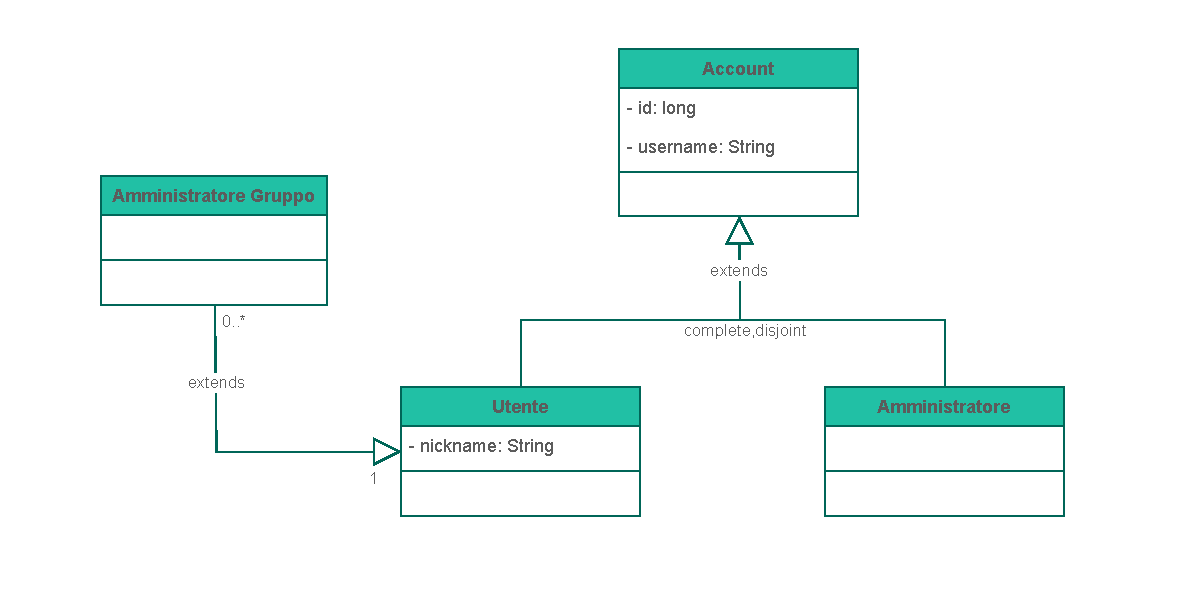
\includegraphics[scale=1]{dominio/Dominio-Struttura Account.drawio.pdf}
\end{adjustwidth}

%------------------------
\pagebreak
\subsubsection*{Area Personale}
\phantomsection
\addcontentsline{toc}{subsection}{Modello del Dominio: Area Personale}
\vspace{0.5cm}
La sezione Area Personale ha come attore l'Utente. Il numero di Viste è limitato a 5. Il numero di File memorizzabili è invece limitato dallo spazio di archiviazione disponibile dall'Utente.\\
L'Utente ha la possibilità di gestire il proprio Account, di caricare, scaricare ed eliminare File e di creare, rimuovere e personalizzare le Viste.\\
\vspace{0.5cm}

\begin{adjustwidth}{-2.5cm}{0cm}
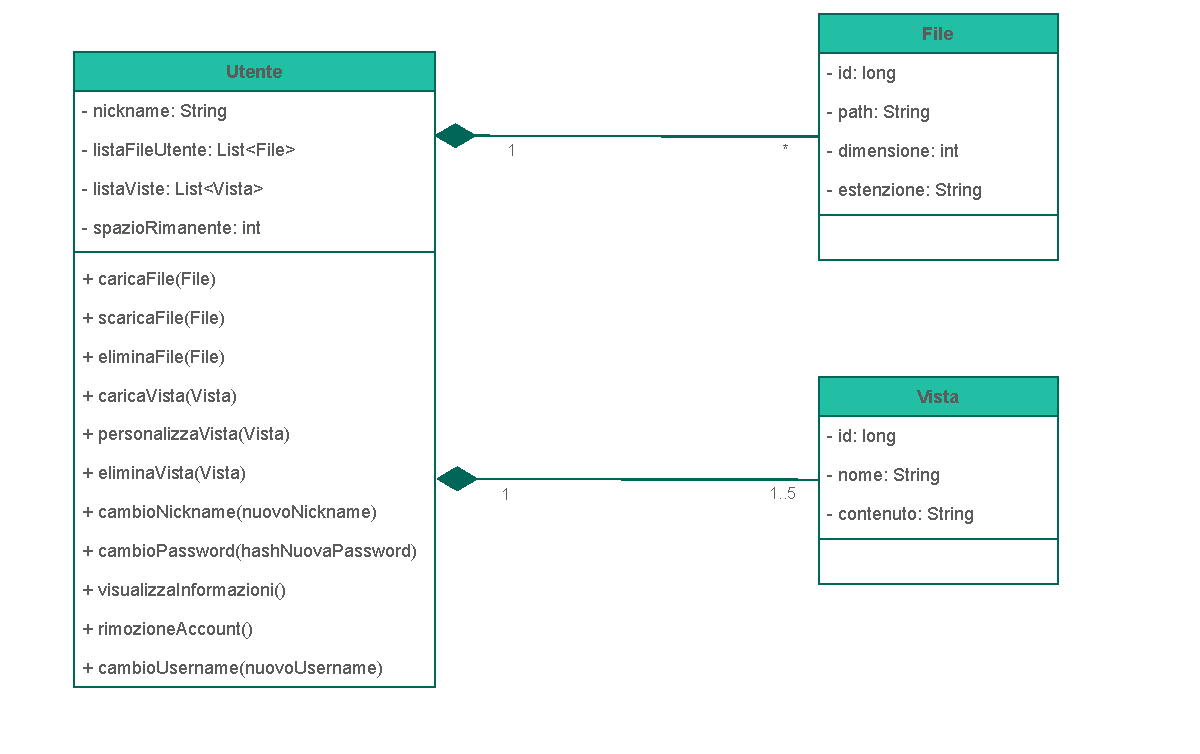
\includegraphics[scale=1]{dominio/Dominio-Area Personale.drawio.pdf}
\end{adjustwidth}


%-----------------
\pagebreak
\subsubsection*{Area Gruppi}
\phantomsection
\addcontentsline{toc}{subsection}{Modello del Dominio: Area Gruppi}
\vspace{0.5cm}
Nell'Area Gruppi, l'Utente ha a disposizione i metodi per accedere ai Gruppi.\\All'interno del Gruppo è possibile visualizzare la lista dei partecipanti e gestire i file di Gruppo.\\Se un Utente è anche Amministratore del Gruppo ha la possibilità di rimuovere i partecipanti dallo stesso.\\
L'Amministratore del gruppo è anch'esso un Utente, necessariamente iscritto a quest'ultimo.
\vspace{1cm}

\begin{adjustwidth}{-3.5cm}{0cm}
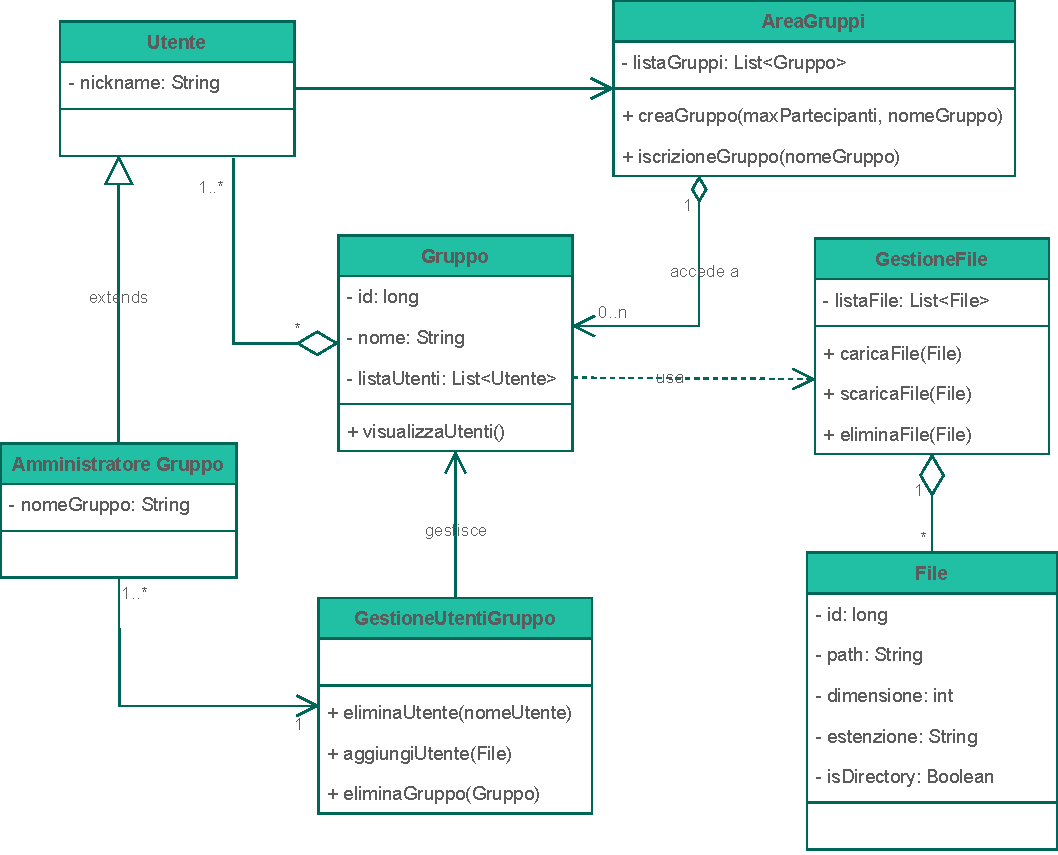
\includegraphics[scale=1]{dominio/Dominio-Area Gruppi.drawio.pdf}
\end{adjustwidth}

%-----------------
\pagebreak
\subsubsection*{Amministrazione}
\phantomsection
\addcontentsline{toc}{subsection}{Modello del Dominio: Amministrazione}
\vspace{0.5cm}

Nella sezione Amministrazione, si dispongono i metodi per gestire le richieste.\linebreak \textbf{gestisciRichiestaUtente()} e \textbf{gestisciRichiestaGruppo()} servono per accettare o rifiutare le richieste "in attesa". \\
L'Amministratore può anche visualizzare la lista degli Utenti registrati e dei Gruppi ed ha la possibilità di rimuoverli.\\
Le operazioni sono tracciate registrando nei Log ogni richiesta.

\vspace{1cm}
\begin{adjustwidth}{-1.5cm}{0cm}
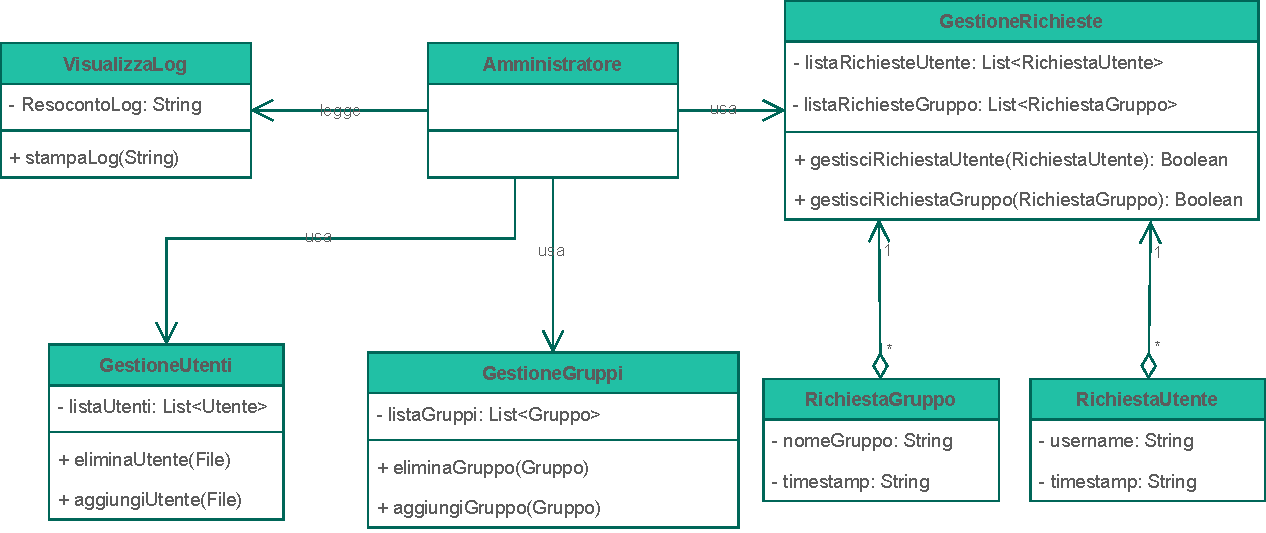
\includegraphics[scale=1]{dominio/Dominio-Amministrazione.drawio.pdf}
\end{adjustwidth}
\pagebreak

%------------------
\phantomsection
\addcontentsline{toc}{section}{Architettura Logica: Struttura}
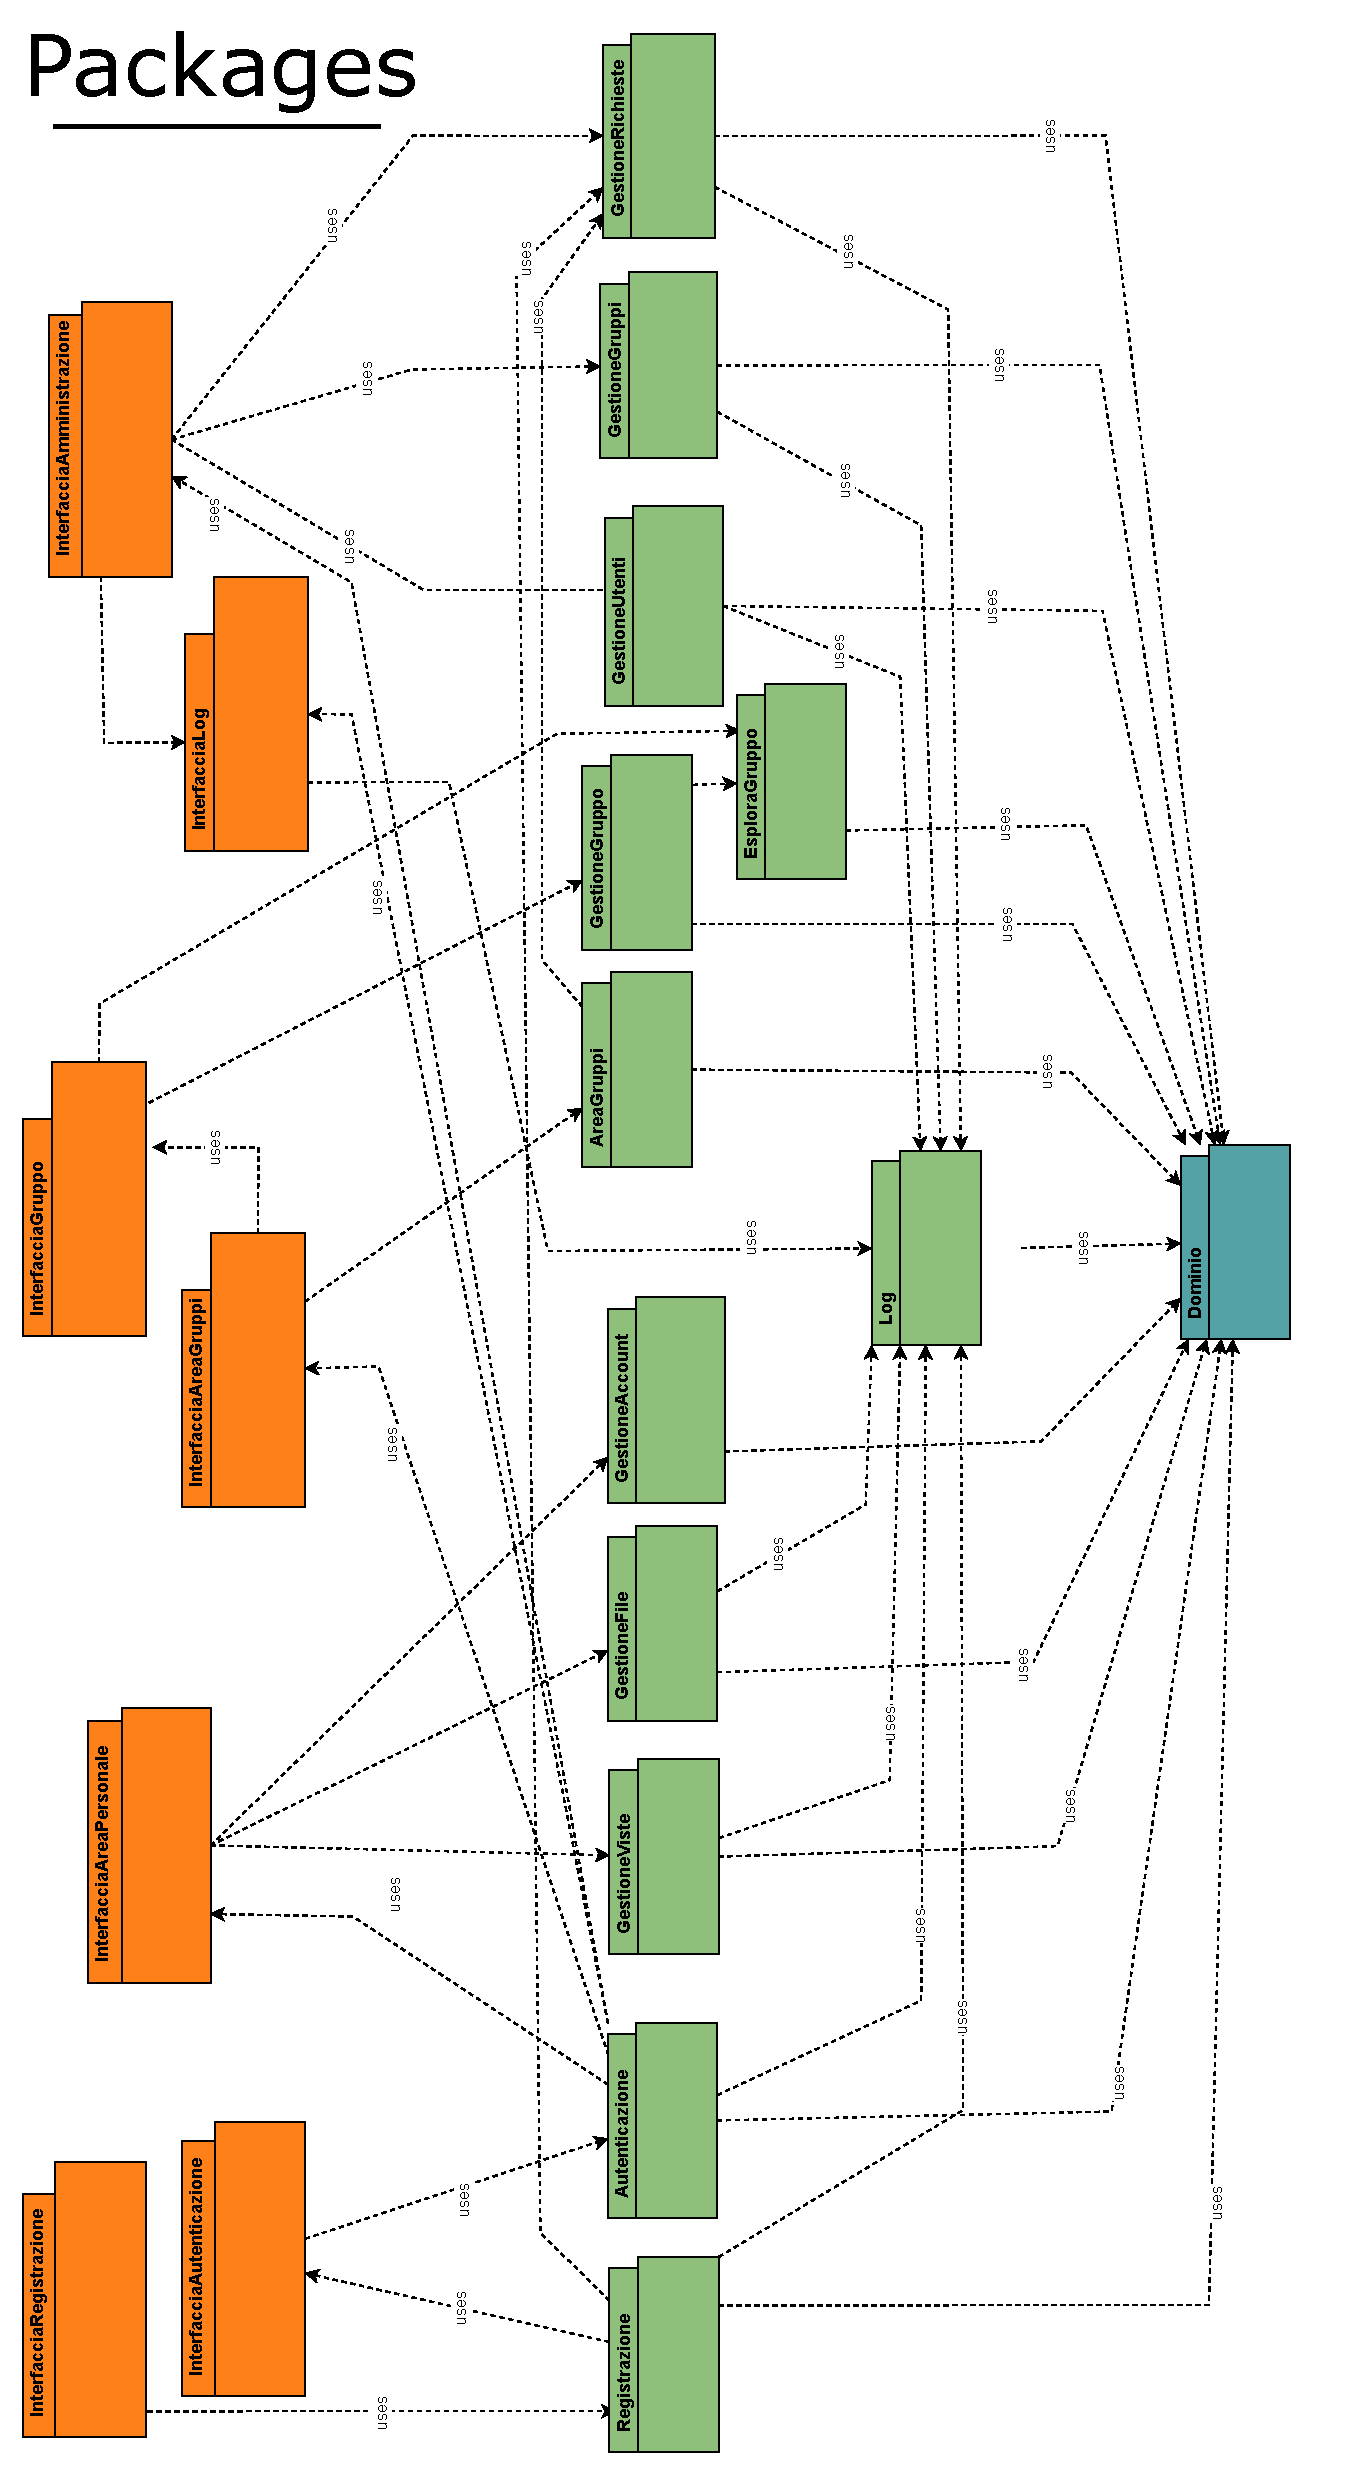
\includepdf[pages={1}]{classi/Package-Package.drawio.pdf}
%-------------------

\subsection*{Diagrammi delle Classi}

\phantomsection
\subsubsection*{Diagramma delle Classi: Autenticazione}
\addcontentsline{toc}{subsection}{Diagramma delle Classi: Autenticazione}
\vspace{1cm}
Il metodo \verb|registraUtente| inserisce la richiesta di registrazione nella \\\verb|listaRichiesteRegistrazione| della classe \verb|GestioneAmministrazioneController|.\\
L'operazione è portata a termine quando l'Amministratore accetta la richiesta.
\vspace{2cm}
\begin{adjustwidth}{-2.5cm}{0cm}
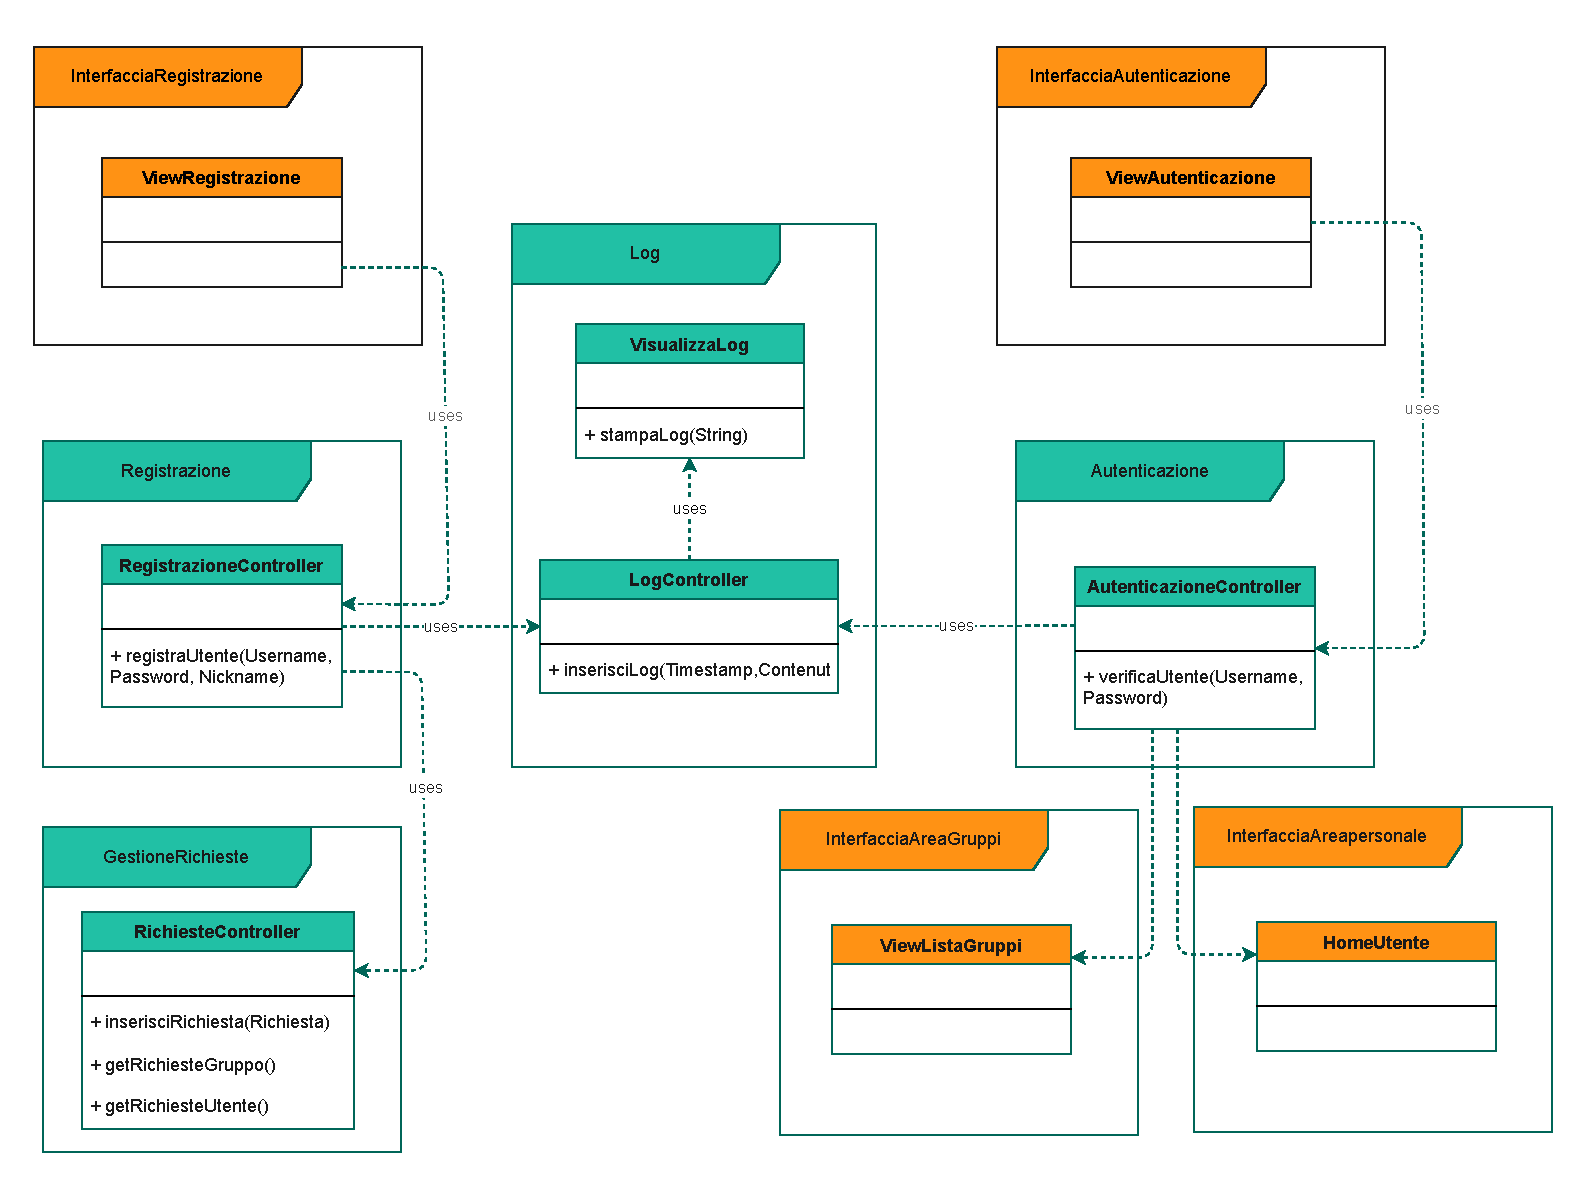
\includegraphics[scale=0.7]{classi/Package-Classi-Autenticazione.drawio.pdf}
\end{adjustwidth}



\phantomsection
\subsubsection*{Diagramma delle Classi: Amministrazione}
\addcontentsline{toc}{subsection}{Diagramma delle Classi: Amministrazione}
\vspace{0.5cm}

\begin{adjustwidth}{-2.5cm}{0cm}
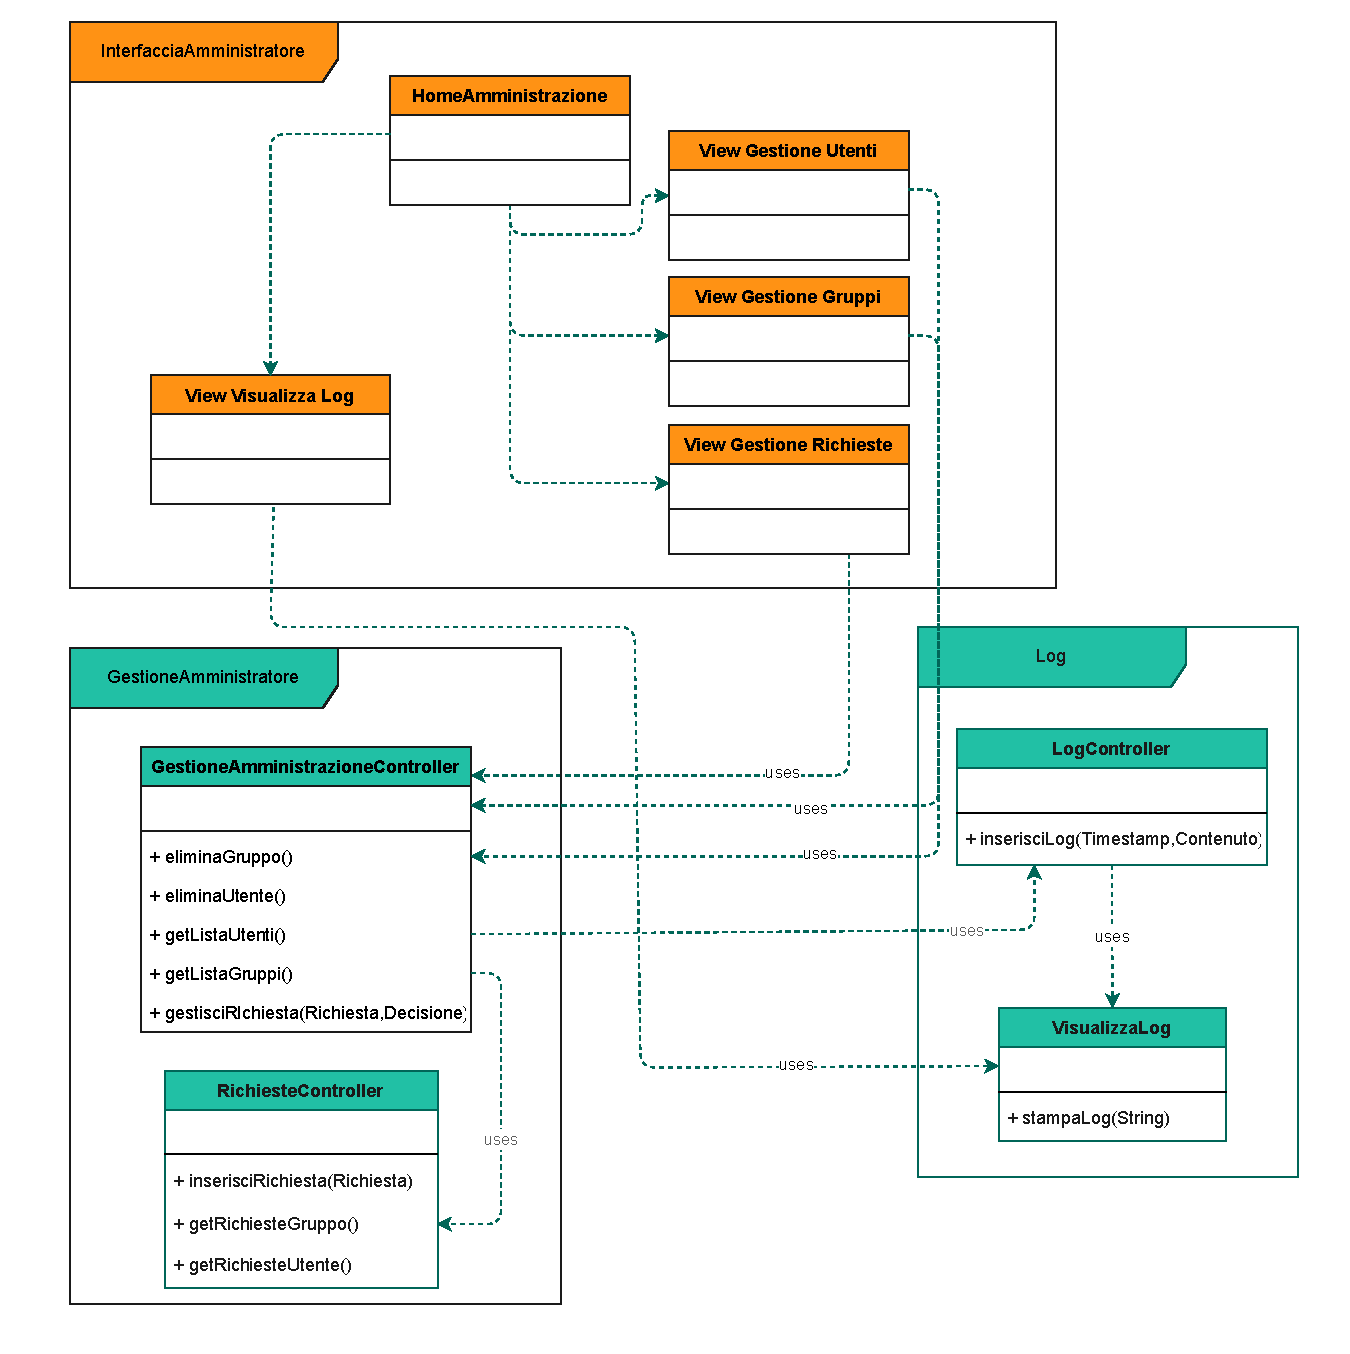
\includegraphics[scale=0.8]{classi/Package-Classi-Amministrazione.drawio.pdf}
\end{adjustwidth}
\pagebreak




\phantomsection
\subsubsection*{Diagramma delle Classi: Utente}
\addcontentsline{toc}{subsection}{Diagramma delle Classi: Utente}
\vspace{0.5cm}

È stato deciso di creare una classe per i File, con un'istanza della classe per ogni File caricato dall'Utente.\\
Questo può essere oneroso per il Server in quanto occupa più memoria, però garantisce una migliore esperienza per l'Utente dato che l'accesso più facile all'alberatura dei file consente una navigazione più immediata.\\

\vspace{0.5cm}
\begin{adjustwidth}{-3.5cm}{0cm}
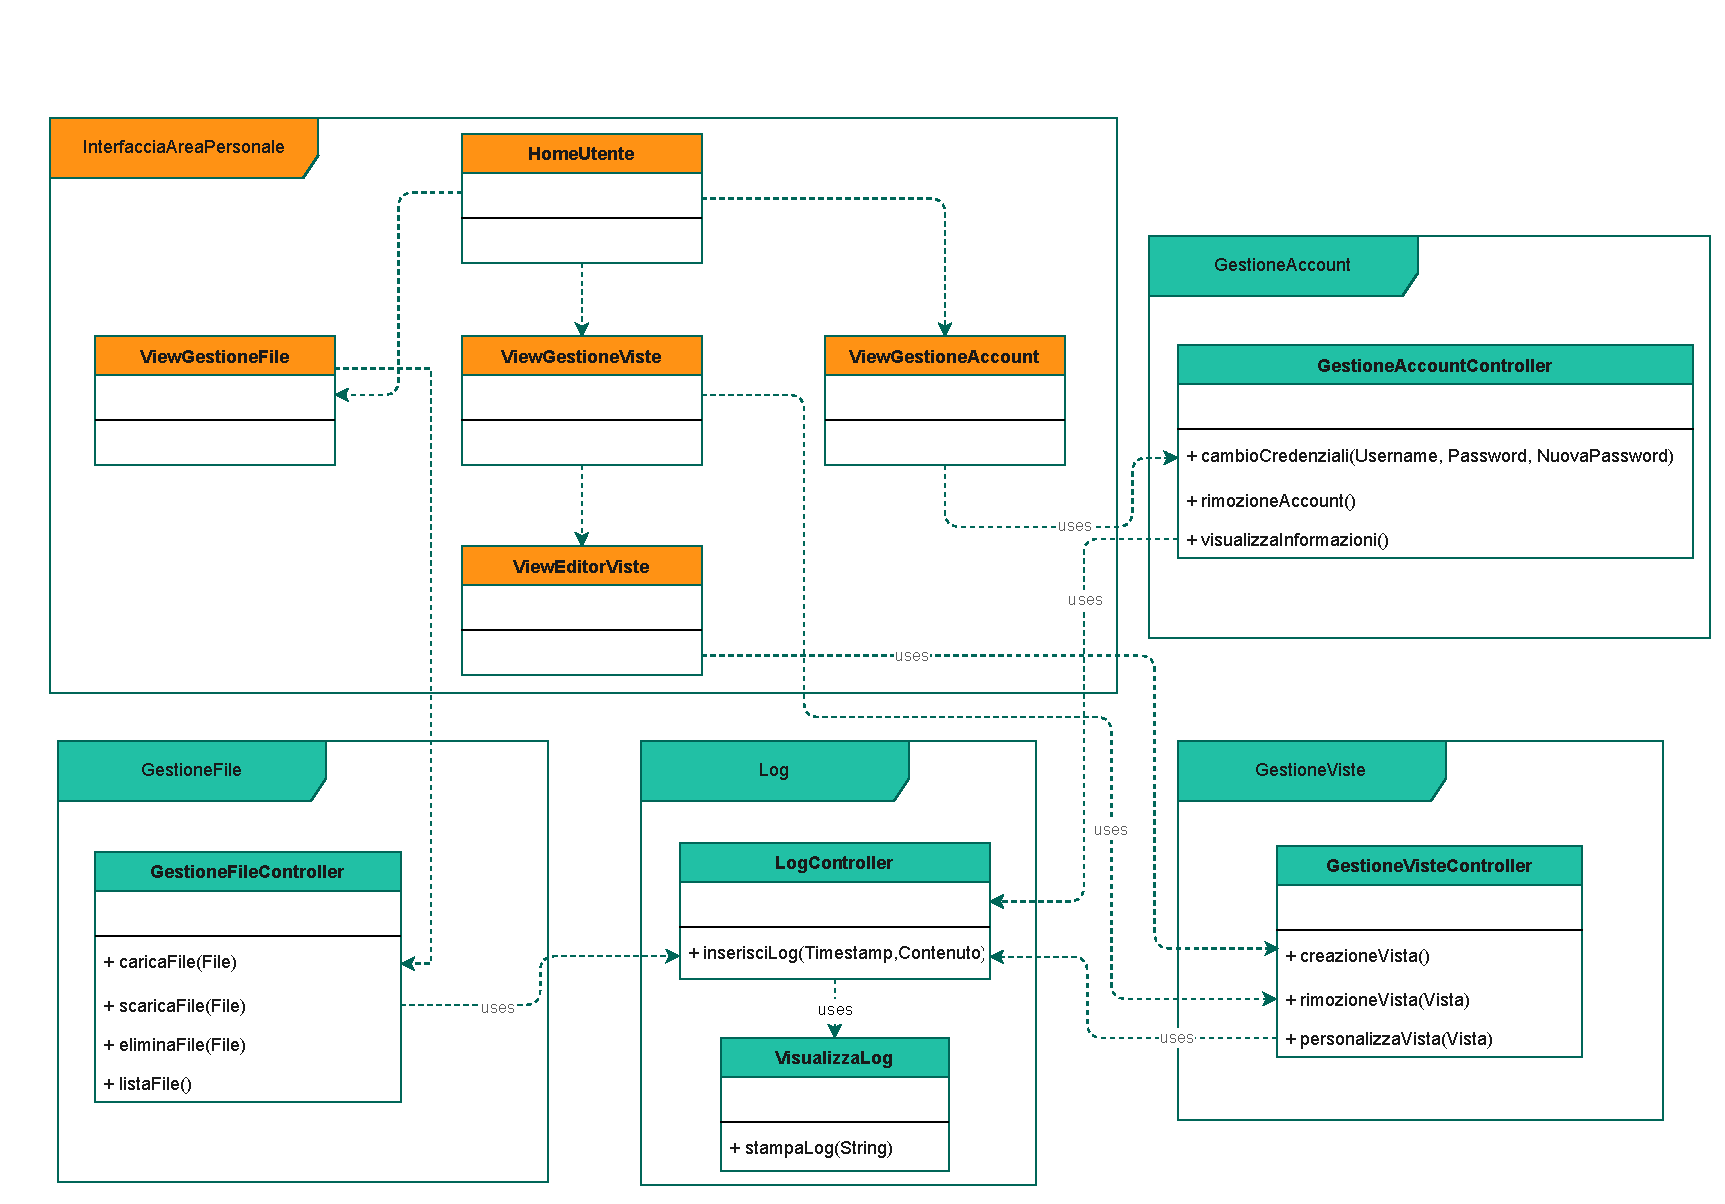
\includegraphics[scale=0.7]{classi/Package-Classi-Utente.drawio.pdf}
\end{adjustwidth}




\pagebreak
\phantomsection
\subsubsection*{Diagramma delle Classi: Gruppi}
\addcontentsline{toc}{subsection}{Diagramma delle Classi: Gruppi}
\vspace{0.5cm}
La creazione di un Gruppo avviene con lo stesso meccanismo di una Registrazione, cioè viene generata una richiesta che sarà poi gestita dall'Amministratore.
\vspace{0.5cm}
\begin{adjustwidth}{-2.5cm}{0cm}
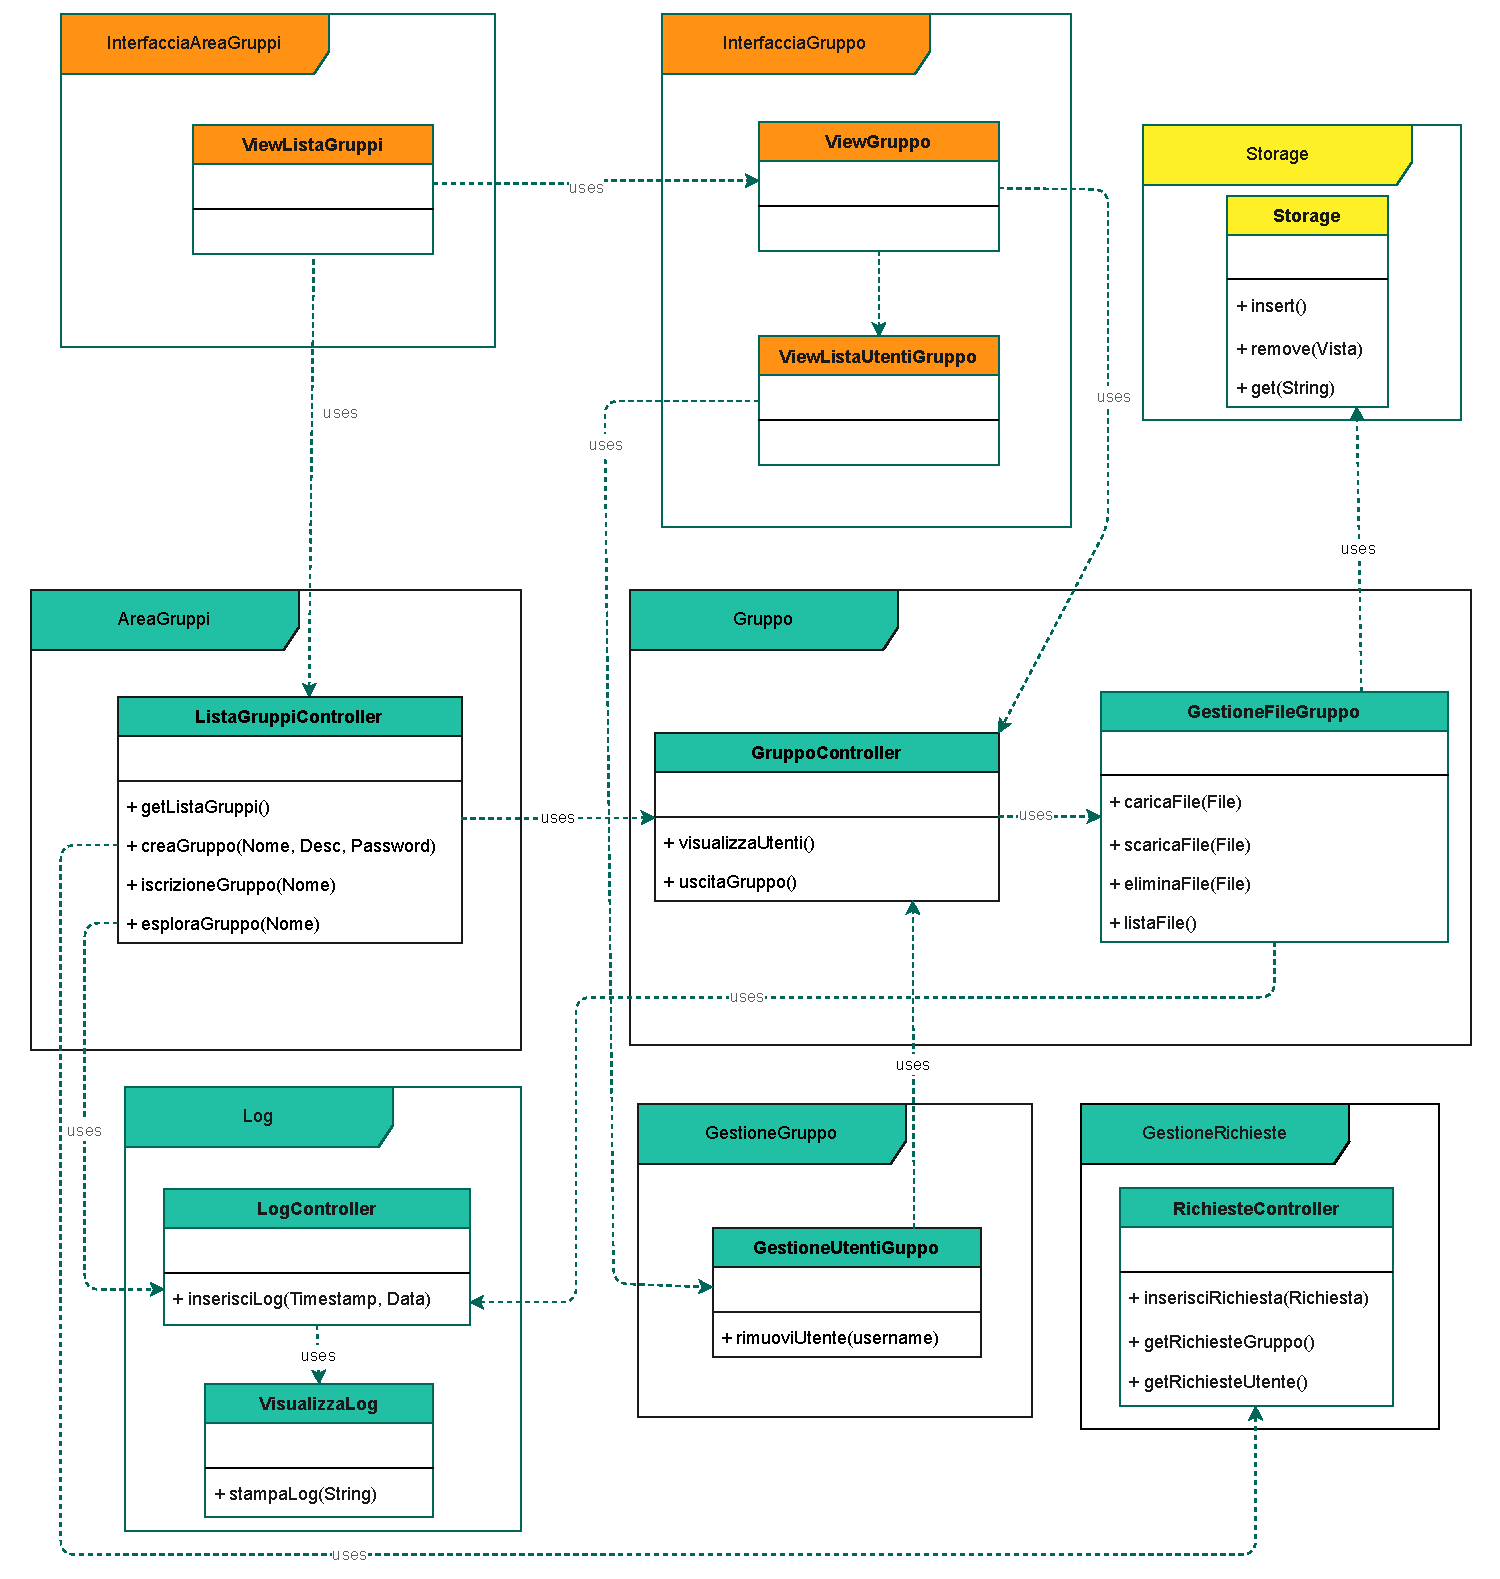
\includegraphics[scale=0.75]{classi/Package-Classi-Gruppi.drawio.pdf}
\end{adjustwidth}



%------------------------------------------


\phantomsection
\section*{Architettura Logica: Interazione}
\addcontentsline{toc}{section}{Architettura Logica: Interazione}
\vspace{0.5cm}


\phantomsection
\subsection*{Diagramma di sequenza : Registrazione}
\addcontentsline{toc}{subsection}{Diagramma di sequenza : Registrazione}
\vspace{0.5cm}

\begin{adjustwidth}{-0.5cm}{0cm}
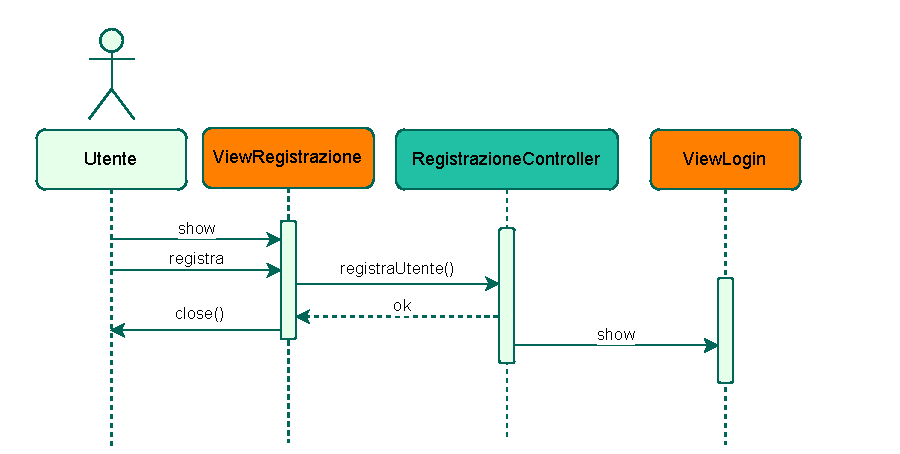
\includegraphics[scale=1]{interazione/Package-Interazione-Registrazione.drawio.pdf}
\end{adjustwidth}

\phantomsection
\subsection*{Diagramma di sequenza : Autenticazione}
\addcontentsline{toc}{subsection}{Diagramma di sequenza : Autenticazione}
\vspace{0.5cm}

\begin{adjustwidth}{1cm}{0cm}
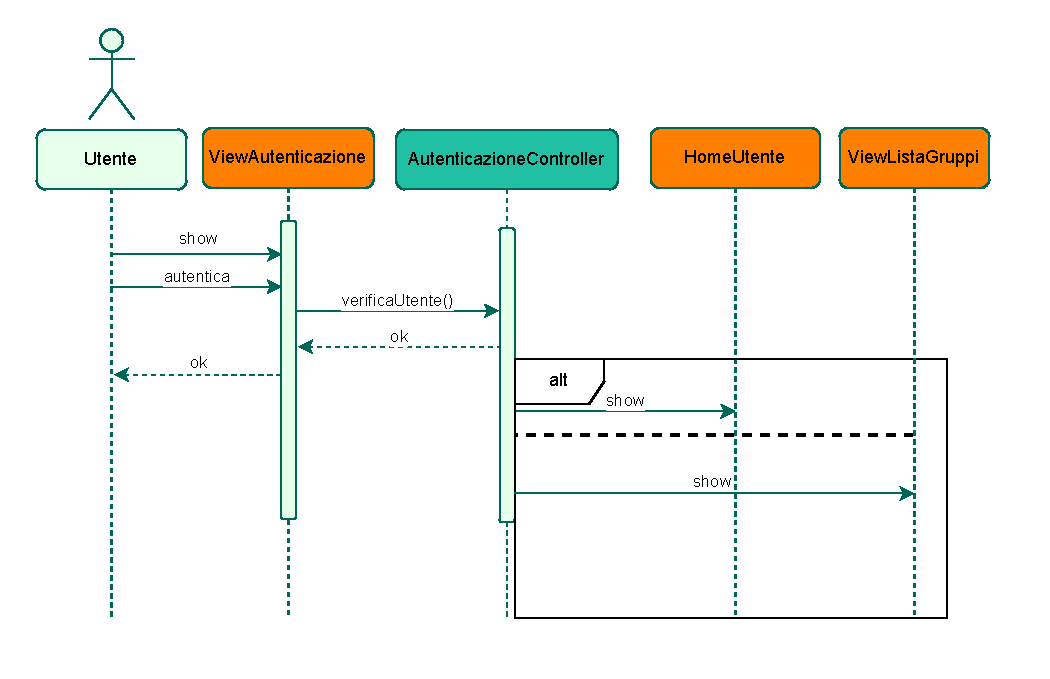
\includegraphics[scale=1]{interazione/Package-Interazione-Autenticazione.drawio.pdf}
\end{adjustwidth}


\phantomsection
\subsection*{Diagramma di sequenza : Gestione Amministratore}
\addcontentsline{toc}{subsection}{Diagramma di sequenza : Gestione Amministratore}


\begin{adjustwidth}{-2cm}{0cm}
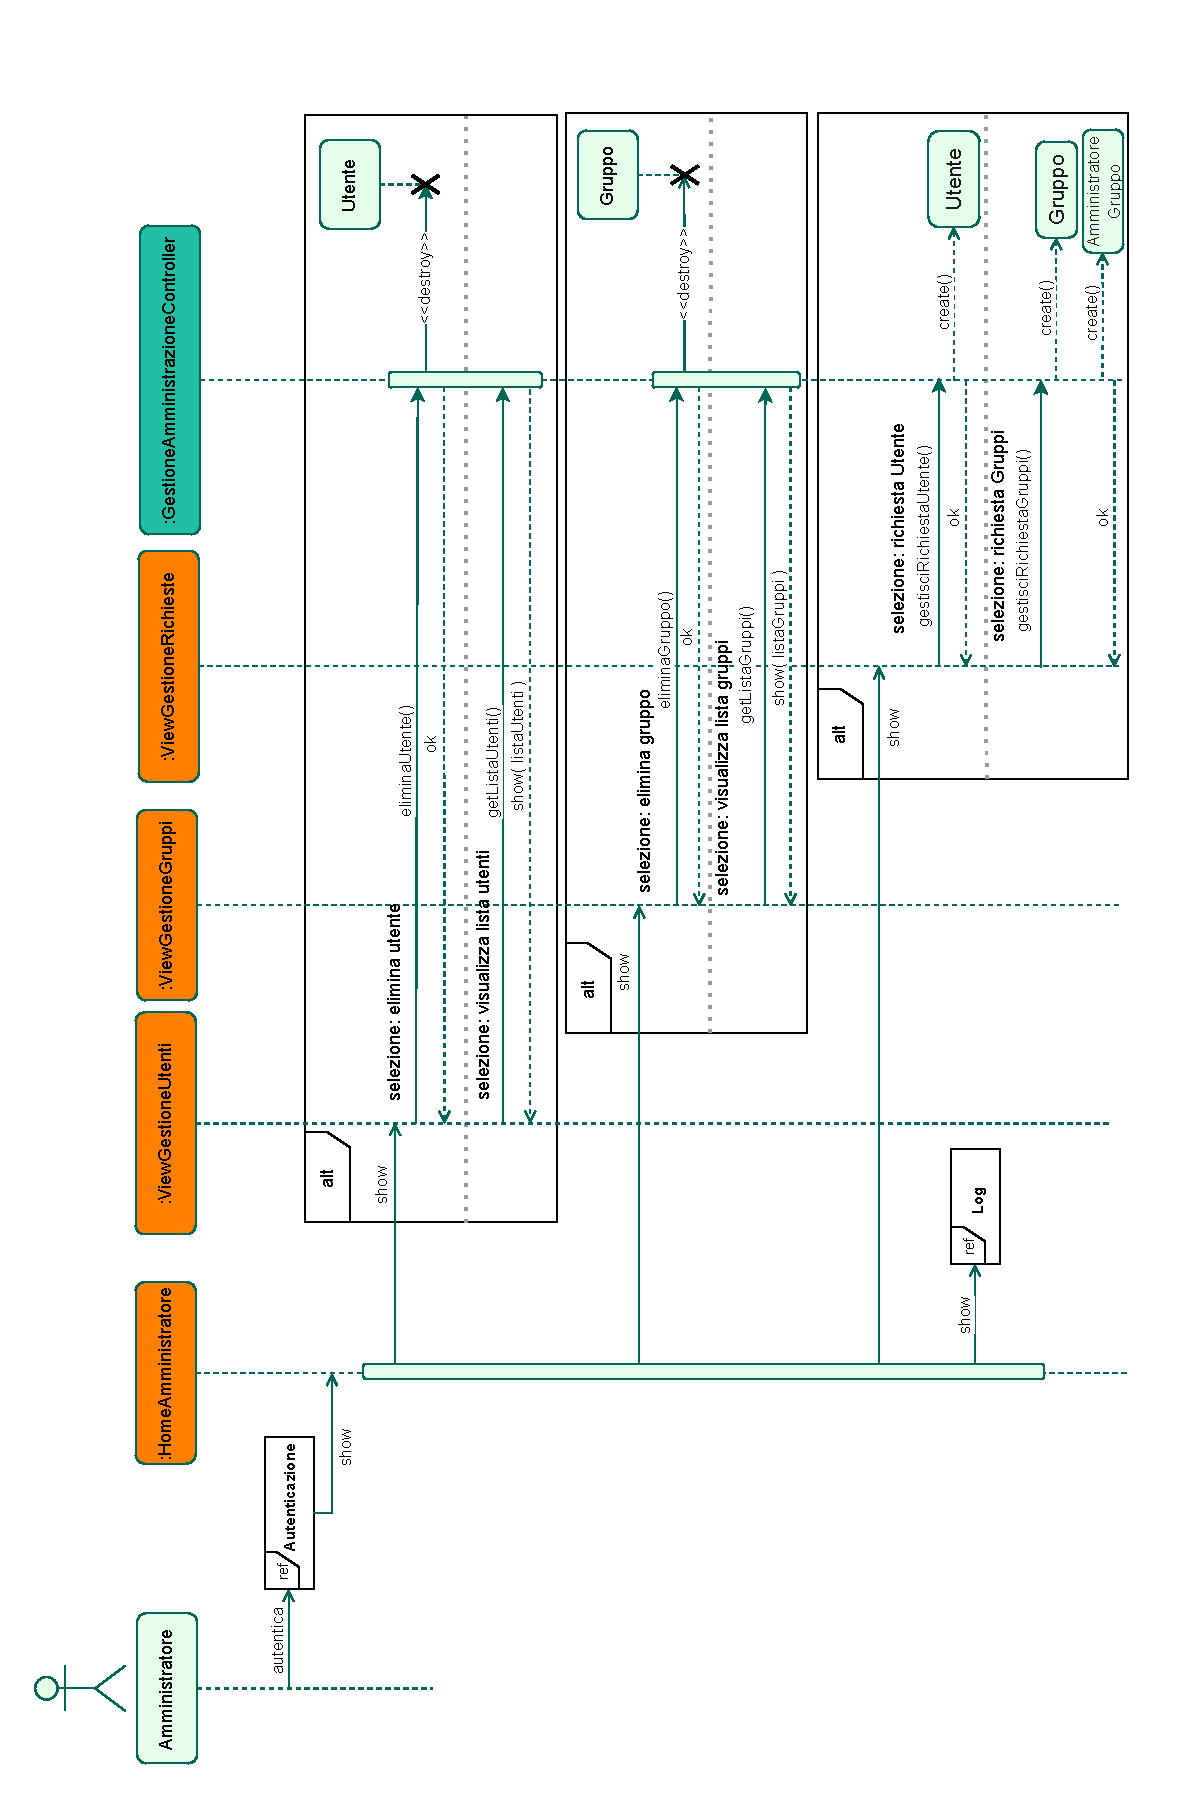
\includegraphics[scale=0.85]{interazione/Package-Interazione-GestioneAmministratore.drawio.pdf}
\end{adjustwidth}

\phantomsection
\subsubsection*{Diagramma di sequenza : Area Personale\-Viste}
\addcontentsline{toc}{subsection}{Diagramma di sequenza : Area Personale\-Viste}
\vspace{0.5cm}

\begin{adjustwidth}{-2cm}{0cm}
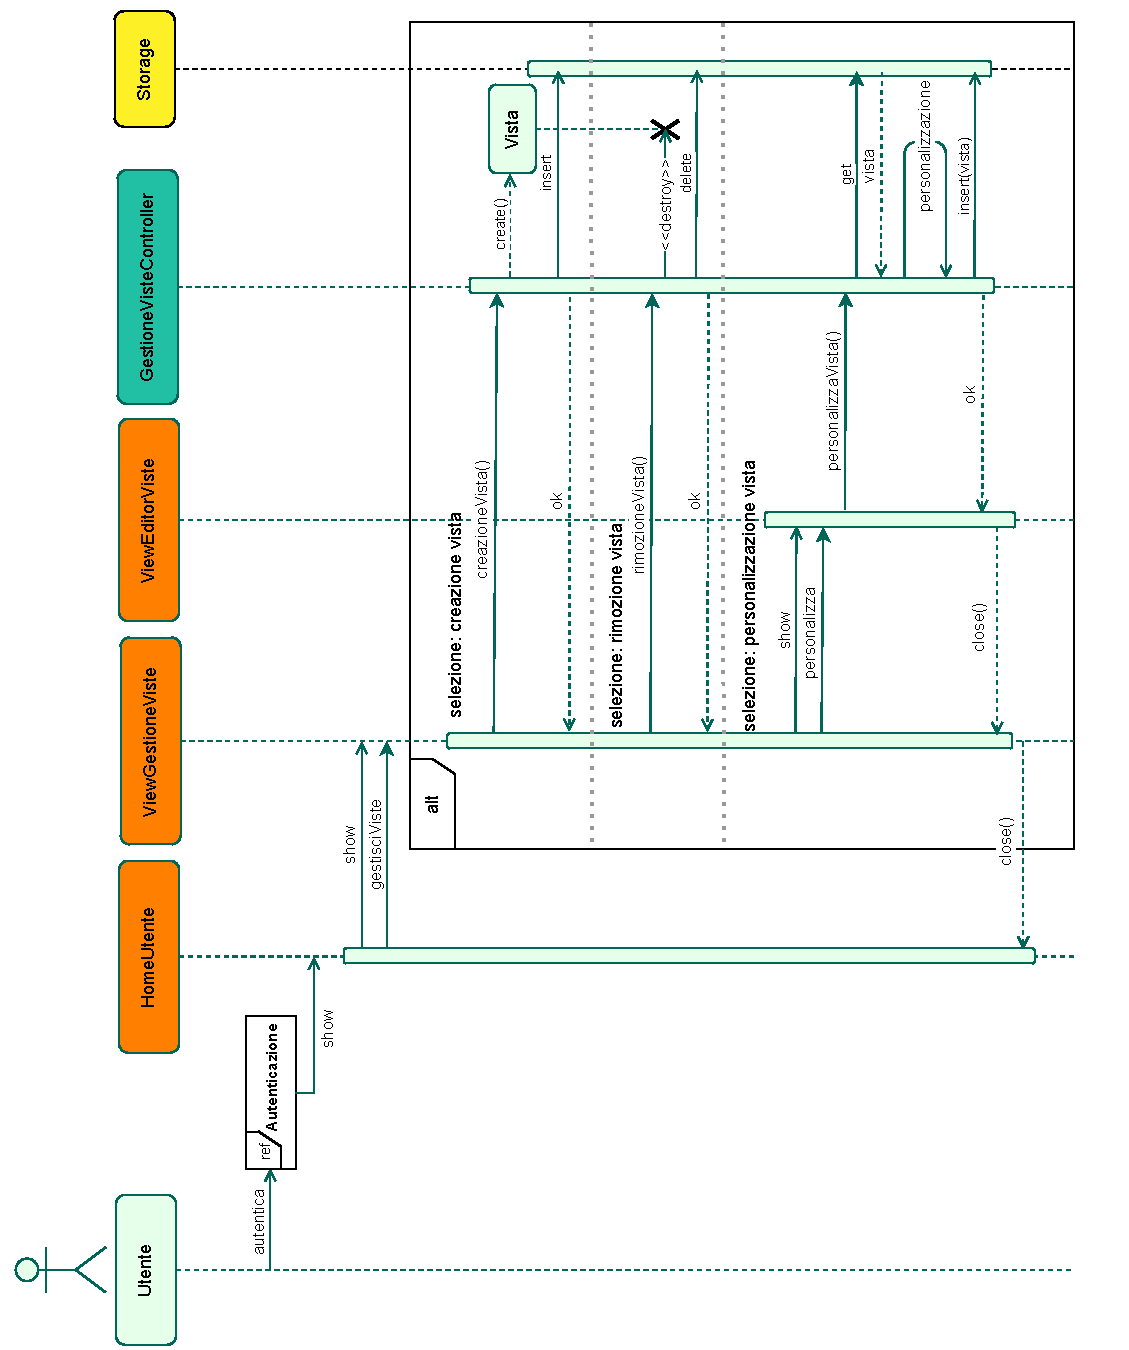
\includegraphics[scale=0.85]{interazione/Package-Interazione-AreaPersonale.drawio.pdf}
\end{adjustwidth}


\phantomsection
\subsubsection*{Diagramma di sequenza : Log}
\addcontentsline{toc}{subsection}{Diagramma di sequenza : Log}
\vspace{0.5cm}

\begin{adjustwidth}{1cm}{0cm}
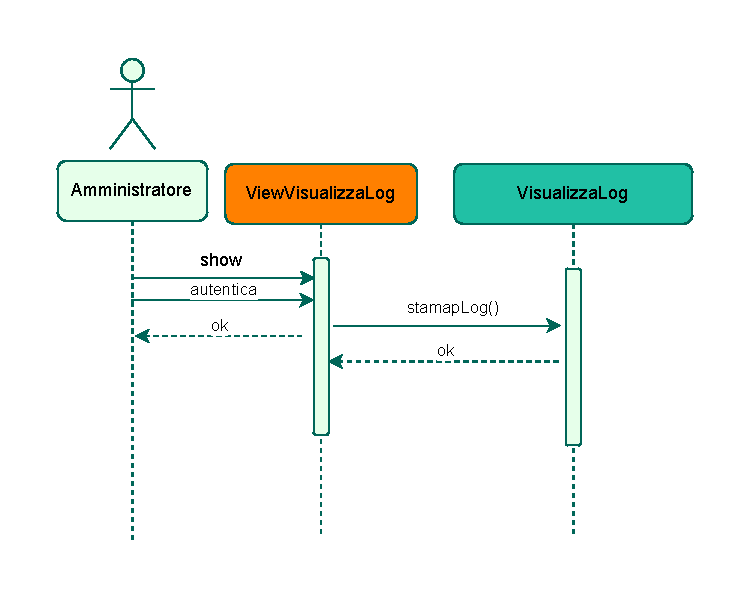
\includegraphics[scale=1]{interazione/Package-Interazione-Log.drawio.pdf}
\end{adjustwidth}
